% ---------
% --------
%!TEX TS-program = pdflatex
%!TEX encoding = UTF-8 Unicode
%!TEX spellcheck = English (Aspell)

\documentclass[11pt]{article}
\usepackage{lucy,handout,graphicx}
\usepackage{fourier-orns}
\usepackage{mathtools}
\usepackage[normalem]{ulem} % either use this (simple) or
\usepackage{tikz}
\usetikzlibrary{graphs}

\allowdisplaybreaks


\begin{document}

\noindent Name \underline{\hspace{12cm}}\\

\begin{center}
\Large\textbf{CSCI 332, Fall 2026}\\
\LARGE\textbf{Exam 1}
\end{center}

\noindent This exam consists of the following sections:
\begin{enumerate}
    \item Stable Matching (25 points)
    \item Algorithm Analysis (25 points)
    \item Recursion (25 points)
    \item Backtracking and 1D Dynamic Programming (25 points)
\end{enumerate}

You may use a double sided 3x5 handwritten notecard of notes during the test but no other resources.

Good luck!

\newpage

\begin{center}
\LARGE\textbf{Section 1 (Stable Matching)\\}%
\end{center}

Questions 1 and 2 refer to the Gale-Shapley algorithm for
stable matching.

    \begin{algo}
    Gale-Shapley(preference lists for $n$ hospitals and $n$ students)\+\\
    Let $M$ be an empty matching\\
    While some hospital $h$ is unmatched and hasn't proposed to every student:\+ \\
        Let $s$ be the first student on $h$'s list to whom $h$ has not yet proposed\\
        If $s$ is unmatched:\+\\
            Add $(h,s)$ to $M$\-\\
        Else $s$ is matched to $h'$:\+\\
            If $s$ prefers $h$ to $h'$:\+\\
                Remove $(h',s)$ from $M$\\
                Add $(h,s)$ to $M$\-\\
            Else $s$ prefers $h'$ to $h$:\+\\
                Do nothing\-\-\-\\
    Return $M$\\
    \end{algo}
\begin{enumerate}


\item (10 points) What is the matching returned by Gale-Shapley for the following input? 

\noindent
\begin{minipage}[t]{0.4\textwidth}
\vspace{0pt}
\centering
\small
\begin{tabular}{c|ccc}
\textbf{Hospital} & \textbf{1st} & \textbf{2nd} & \textbf{3rd} \\
\hline
$h_1$ & $s_1$ & $s_2$ & $s_3$ \\
$h_2$ & $s_1$ & $s_2$ & $s_3$ \\
$h_3$ & $s_2$ & $s_3$ & $s_1$ \\
\hline
\textbf{Student} & \textbf{1st} & \textbf{2nd} & \textbf{3rd} \\
\hline
$s_1$ & $h_3$ & $h_2$ & $h_1$ \\
$s_2$ & $h_1$ & $h_2$ & $h_3$ \\
$s_3$ & $h_1$ & $h_2$ & $h_3$ \\
\end{tabular}
\end{minipage}\hfill
\begin{minipage}[t]{0.57\textwidth}
\vspace{0pt}
\small
\textbf{Choose the matching returned:}
\begin{enumerate}[(a)]
    \item \shortstack[l]{$\{(s_1,h_2),(s_2,h_1),(s_3,h_3)\}$}
    \item \shortstack[l]{$\{(s_1,h_3),(s_2,h_1),(s_3,h_2)\}$}
    \item \shortstack[l]{$\{(s_1,h_1),(s_2,h_2),(s_3,h_3)\}$}
    \item \shortstack[l]{$\{(s_1,h_2),(s_2,h_3),(s_3,h_1)\}$}
\end{enumerate}
\end{minipage}

\item (5 points) Does a distinct stable matching exist for this input? Circle: Yes or No.
\\
The input is copied again in case that is useful.


\begin{table}[h]
\centering
\begin{tabular}{c|ccc}
\textbf{Hospital} & \textbf{1st choice} & \textbf{2nd choice} & \textbf{3rd choice} \\
\hline
$h_1$ & $s_1$ & $s_2$ & $s_3$ \\
$h_2$ & $s_1$ & $s_2$ & $s_3$ \\
$h_3$ & $s_2$ & $s_3$ & $s_1$ \\
\hline
\textbf{Student} & \textbf{1st choice} & \textbf{2nd choice} & \textbf{3rd choice} \\
\hline
$s_1$ & $h_3$ & $h_2$ & $h_1$ \\
$s_2$ & $h_1$ & $h_2$ & $h_3$ \\
$s_3$ & $h_1$ & $h_2$ & $h_3$ \\
\end{tabular}
\end{table}

\item (5 points) Is it true that in every input to the stable matching problem, if a
hospital $h$ ranks a student $s$ first and that same student $s$ ranks that same
$h$ first, then $(h,s)$ is matched in every possible stable matching of this input?
Circle True or False.

\item (5 points) Is it true that every stable matching contains at least one pair $(h,s)$
so that $h$ ranks $s$ first and $s$ ranks $h$ first?
Circle True or False.

\newpage

\begin{center}
\LARGE\textbf{Section 2 (Algorithm Analysis)\\}%
\end{center}

\item (5 points)
Order the following functions from asymptotically smallest to asymptotically
largest by labeling the smallest with a 1 and increasing from there.  \textbf{If two
functions are asymptotically equal (one is $\Theta$ of the other), give them the
same number}. Two are filled as an example for you.

    \begin{itemize}
        \item[\underline{\hspace{0.5cm}}] $\log_4 n^3$
        \item[\underline{\hspace{0.5cm}}] $n + \log n$
        \item[\underline{\makebox[0.5cm][c]{1}}] $100^{100!}$
        \item[\underline{\makebox[0.5cm][c]{1}}] $5$ 
        \item[\underline{\hspace{0.5cm}}] $\log_{10} 100^{10}$
        \item[\underline{\hspace{0.5cm}}] $\log_2 n$
    \end{itemize}


    \item (5 points) Select all functions $f(n)$ such that the runtime of
Algorithm-1 below is $\Theta(f(n))$.

    \begin{algo}
    Algorithm-1(array $A$ of length $n$):\+\\
    Result = 0\\
    For each $i$ in $1$ to $n$:\+\\
    For each $j$ in $1$ to $i$:\+\\
    Set Result to $A[j]$ times Result\-\- \\
    Return Result\\
    \end{algo} 

\begin{enumerate}[A.]
    \item $n$
    \item $\log n$
    \item $n^2$
    \item $n^3$
    \item $n!$
\end{enumerate}

\item (5 points) Recall that the definition of big O is as follows:
\emph{$f(n)$ is $O(g(n))$ if there exist positive constants $c$ and $n_0$ such
that for all $n \geq n_0$, $f(n) \leq c \cdot g(n)$.} Select all pairs $n_0$ and $c$ can be
used to show that $4n + 10$ is $O(n)$.
\begin{enumerate}[A.]
    \item $n_0 = 1$, $c = 4$
    \item $n_0=10, c = 4$
    \item $n_0 = 10$, $c = 5$
    \item $n_0 = 1$, $c = 1000$
    \item $n_0 = 100$, $c = 1$

\end{enumerate}

\item
(5 points)
Suppose you know that an algorithm has a best-case runtime that is $O(n^2)$. For each of the following, decide whether it is definitely true, definitely false, or could be true or false and circle your choice. 

\begin{itemize}
    \item The algorithm's worst-case runtime is $\Omega(n)$. T, F, T or F
    \item The algorithm's worst-case runtime is $\Omega(n^3)$. T, F, T or F
    \item The algorithm's best-case runtime is $O(n^3)$. T, F, T or F
\end{itemize}
\newpage


\item (5 points)
You suspect that in the most recent update to your favorite software package,
the implementation of your favorite function \texttt{do-stuff} was replaced by a $\Theta(n^2)$ 
algorithm, whereas it was a $\Theta(n^3)$ algorithm before. Whatever the runtime is, you know that
it is the same for all input classes (that is, the worst case and best case runtimes are equal).
Unfortunately, the package is
closed-source and you cannot inspect the source code; you can only run the function on
various-sized inputs and record its runtime on those inputs.

Describe an experiment that you could run to verify your hunch. That is, tell us what kinds
of input sizes you will run \texttt{do-stuff} on and how you will use their runtimes to
determine whether the algorithm is $\Theta(n^2)$ or $\Theta(n^3)$.




\newpage

\begin{center}
\LARGE\textbf{Section 3 (Recursion)\\}%
\end{center}
 
\item (15 points)

Consider the recurrence $T(n) = 2T(n/3) + n^3, T(1) = 1$.

\begin{enumerate}[(a)]

\item (5 points) In the left boxes, draw the first three levels of this recursion tree.
In the boxes next to them, write the total work on that level.

\begin{center}
\begin{tikzpicture}[
  boxL/.style={draw, rectangle, minimum width=9cm, minimum height=2.2cm, inner sep=6mm},
  boxR/.style={draw, rectangle, minimum width=4.1cm, minimum height=2.2cm, inner sep=6mm},
  smalllabel/.style={font=\scriptsize, anchor=north west}
]

\node[boxL] (L0) at (0,4.0) {};
\node[smalllabel] at (L0.north west) {Level 0};

\node[boxL] (L1) at (0,1.5) {};
\node[smalllabel] at (L1.north west) {Level 1};

\node[boxL] (L2) at (0,-1) {};
\node[smalllabel] at (L2.north west) {Level 2};

\node[boxR] (R0) at (7,4.0) {};
\node[smalllabel] at (R0.north west) {Sum level 0};

\node[boxR] (R1) at (7,1.5) {};
\node[smalllabel] at (R1.north west) {Sum level 1};

\node[boxR] (R2) at (7,-1) {};
\node[smalllabel] at (R2.north west) {Sum level 2};

\end{tikzpicture}
\end{center}
\item (3 points) What is the work per level in terms of level $\ell$?
\vspace{1in}
\item (2 points) Is the work per level (circle one)
\begin{itemize}
    \item increasing (work is dominated by leaves)
    \item decreasing (work is dominated by root)
    \item the same (work is the same at every level)
\end{itemize}
\item (3 points)  What is the total number of levels in the tree? (fill in the base and the argument of the logarithm)
\[
\text{number of levels} = \log_{\underline{\hspace{1cm}}}(\underline{\hspace{1cm}})
\]

\item (2 points) What is the closed-form (non-recursive form) of $T(n)$?
\vspace{1in}
\end{enumerate}
\newpage
Recall the algorithm for binary search:
\begin{algo}
    \underline{BinarySearch(sorted $A[1..n]$, $t$):}\+ \\
    $\ell = 1, r = n$\\
    while $\ell \leq r$: \+ \\
    $m = \floor{\frac{\ell + r}{2}}$\\
    if $A[m] > t$: \Comment{go left}\+ \\
    $r = m - 1$ \- \\
    else if $A[m] < t$: \Comment{go right} \+ \\
    $\ell = m + 1$ \-\\
    else: \Comment{equal}\+ \\
    return $m$\- \- \\
    return $-1$
\end{algo}
In this problem, you will instead solve the following problem:
Suppose you are given a sorted array of n distinct numbers that has been
rotated k steps, for some unknown integer $k$ between $1$ and $n-1$. That is,
you are given an array $A[1..n]$ such that some prefix $A[1..k]$ is sorted in
increasing order, the corresponding suffix $A[k + 1..n]$ is sorted in increasing
order, and $A[n]$ < $A[1]$.  For example, you might be given the following $16$-element
array (where $k = 10$):
\begin{center}
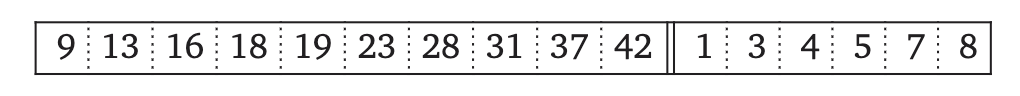
\includegraphics[width=.8\textwidth]{array.png}
\end{center}
Your task is to determine what $k$ is in $O(\log n)$ time.
\item (10 points) You will still look at the midpoint $m$ between your current $\ell$ and $r$
indices in the array. How will you decide whether to go left or right?

\newpage


\begin{center}
\LARGE\textbf{Section 4 (Backtracking and 1D Dynamic Programming)\\}%
\end{center}

    In your country, there are only coins of denominations 1, 3, and 4. You
    would like to write an algorithm to solve the following problem: Given a
    positive integer $n$, what is the fewest number of coins you can use to
    represent $n$?

    To solve this problem, you choose the following English definition of the recursive subproblems.

     \textbf{Let $MinCoins(i)$ be the minimum number of coins needed to represent the amount $i$.}

     \item (2 points) What is $MinCoins(6)$?

     \vspace{1in}

     \item (8 points) Write the recursive definition for $MinCoins(i)$. You may not need every line provided.

    \begin{equation*}
        MinCoins(i) =
        \begin{cases}
        \underline{\hspace{3.5in}} & if i \underline{\hspace{.5in}} \\
        \underline{\hspace{3.5in}} & if i \underline{\hspace{.5in}} \\
        \underline{\hspace{3.5in}} & if i \underline{\hspace{.5in}} \\
        \underline{\hspace{3.5in}} & if i \underline{\hspace{.5in}} \\
        \underline{\hspace{3.5in}} & if i \underline{\hspace{.5in}} \\
        \end{cases}
    \end{equation*}
    \newpage

    Given the following (meaningless) recursive definition of a subproblem
\begin{equation*}
    doh(i) =
    \begin{cases}
        4 & if i = n \\
        $H[n-1]$ & if i = n-1\\
        0 & if i = n-2\\
        \min \left(2\cdot H[i] + doh(i+1), doh(i+3)\right) & if i < n-2 \\

    \end{cases}
\end{equation*}

    \item (2 points)
    We can store solutions to the subproblems in an array. What direction should we fill it (left to right or right to left)?
    \vspace{1in}

    \item (8 points)

    Using the above information, finish the pseudocode
    to compute $doh(1)$ for a 
    given $H[1..n]$.
    \begin{algo}
    MemoizedDoh($H[1..n]$):\+\\
    Let array $M$ be an array of length $n$\\
    \# do we have any base cases?\\
    \\
    \\
    \\
    \\
    \\
    \# how should we fill in the rest of the array?\\
    \\
    \\
    \\
    \\
    \\
    \\
    \\
    \\
    \# what should we return to get the final answer?\\
    \\
    \\
    \\
    \hspace{5in}
    \end{algo}

    \newpage
    The subset-sum problem is as follows:
    Given a set $X$ of positive integers and a target integer $T$, is there
    a subset of elements in $X$ that add up to $T$? For example, if $X=\Set{8, 6, 7, 5, 3, 10, 9}$
    and $T=15$, the answer is True, because the subsets $\Set{8,7}$ and $\Set{6,9}$ and $\Set{7, 5, 3}$
    all sum to 15.


    \item (1 point) 
    Find one more subset that sums to 15 in $X$.
    \vspace{1in}

    \item (4 points) Consider the following subproblem: \textbf{Let $SubsetSum(S,
    t)$ be True if the set S contains a subset that sums to $t$ and False if
    not.} To write the recursive case of a backtracking algorithm to
    solve subset-sum, we observe that if we have a set $S$ and a target $t$, we
    can remove any single element $x$ from $S$. Then, our recursive algorithm should explore
    two choices, \textbf{which you should state as new calls to SubsetSum()}. Make sure you specify
    the two parameters that SubsetSum takes in.
    \begin{itemize}
        \item Choice 1:
        \vspace{1in}
        \item Choice 2:
        \vspace{1in}
    \end{itemize}


\end{enumerate}
\end{document}
